\chapter{层网格剖分}

增材制造工艺仿真的残余应力和变形计算中,可以分为小尺度和构件尺度,小尺度考虑热循环细节,采用生死单元法,构件尺度忽略热循环细节,采用固有应变法。生死单元法中需要根据热源移动激活网格单元,采用静单元和激活单元的混合方法。热源是根据事先规划好的路径进行移动,路径是逐层规划的,因此对网格剖分提出了特殊的要求,网格单元需要在一层。固有应变法也需要对网格进行分块。因此我们针对增材制造特殊要求,整理计算几何中网格剖分算法,在现有层网格剖分软件基础上实现自适应和并行,并比较Delaunay网格和像素网格的效果。计算几何请参考\cite{JeanMarietteHerve}、\cite{JakobJensFrançoisHenrik}和\cite{MarkMarcMarkOtfried},网格剖分请参考\cite{PascalPaul}和\cite{PaulHouman},计算机辅助设计(CAD)请参考\cite{Erich}。

\section{非结构性网格}

网格剖分包括结构性网格和非结构性网格,结构性网格剖分主要包括Algebraic Interpolation Method和PDE-based Methods,Algebraic Interpolation Method通过映射将简单形状转成复杂形状,非结构性网格剖分主要包括Spatial Decomposition Method、Advancing-front Method、Delaunay Technique,网格剖分还可以分为二维网格剖分、三维网格剖分和三维曲面网格剖分,三维曲面网格剖分可以采用结构性网格剖分映射类方法,也可以采用非结构性网格的剖分方法。增材制造层网格剖分由于网格逐层增加,和Advancing-front Method非常类似,可以通过设置推进距离满足层网格要求,区别在于三维实体模型是通过切片定义还是通过边界网格定义。根据切片定义,CNR IMATI的团队采用了层二维剖分到三维,我们对该方法进行研究并和其他方法进行比较。路径规划方法可以借鉴网格剖分,分为二维、三维和三维曲面,分为等距线、等距面、截平面,二维等距线可以采用法向等距或者费马螺旋曲线等距,三维等距面可以采用法向等距,法向等距类似Advancing-front Method,例如infill和offset,三维曲面路径可以采用映射也可以采用测地线等距,或者截平面,测地线等距类似Advancing-front Method,需要微分几何的知识。

首先看Delaunay网格剖分,狄利克雷镶嵌(Dirichlet Tessellation),沃罗诺伊图(Voronoi Diagram)和德劳内三角网格(Delaunay Triangulation)是网格剖分的基本概念。狄利克雷首先提出了可以将平面分割成凸单元,其次沃罗诺伊进行了进一步研究,并扩展到三维,最后德劳内验证了可以通过沃罗诺伊图的对偶获取三角网格,这种三角网格具有唯一性和很好的性质,最小角比其他存在的三角网格的最小角都大。沃罗诺伊图定义中单元和点集中某一点对应,单元中的点离该点距离比离点集其他点都近,如果是二维问题就是由连接两邻点直线的垂直平分线围成的多边形。德劳内三角网格生成有不同方法,可以根据沃罗诺伊图对偶生成,比较常用的是递增法(Incremental Method),递增法是基于德劳内引理。德劳内引理证明了如果对于每对相邻单形都满足空外接圆准则,那么整个网格满足空外接圆准则并且是德劳内三角网格。基于德劳内引理,定义德劳内核,德劳内核原理是往旧网格中插入一点,如果该点在某一网格单元内,将该点和网格单元三个顶点连线,如果该点在网格单元某一边相邻网格单元外接圆内,则将该边进行翻转,从而获取新网格。插入点还有落在所有网格单元外的情况,为了避免这种情况,采用了一个技巧(Reduced Incremental Method),定义一个盒子包括了整个点集。我们对主要开源网格剖分软件中的数据结构和算法进行研究,包括CGAL、Triangle、Netgen、Tetgen、Gmsh、OpenCASCADE,OpenCASCADE是CAD软件也需要表面网格剖分,从而形成了非结构性层网格剖分框架。

\subsection{CGAL}

\subsubsection{数据结构和算法}
CGAL是一个重模板的软件,新版本程序全部都写在头文件中,因此不需要编译。CGAL中包括二维和三维的点集生成三角网格(Triangulation),包括二维和三维的网格剖分(Mesh Generation),两者的区别是网格剖分是在点集生成的三角网格基础上根据网格质量准则进一步处理,比如进行德劳内加密。在三维网格剖分中有周期性网格剖分,后边将测试是否可以用于层网格剖分。CGAL中二维点集生成三角网格有四个算法,分别为Triangulation\_2、Delaunay\_triangulation\_2、Constrained\_triangulation\_2、Constrained\_Delaunay\_triangulation\_2,还有一些其他算法,程序在Triangulation\_2文件夹中。第二个算法和第三个算法基于第一个算法,第四个算法基于第三个算法,第一个算法实现了点递增插入,第二个算法增加了翻转,第三个算法增加了约束,第四个算法增加了翻转和约束。通常来说网格数据结构包括顶点坐标和单元编号两部分,在这四个算法中默认定义的数据结构是Triangulation\_data\_structure\_2,程序在TDS\_2文件夹中。Triangulation\_data\_structure\_2中采用了两个Compact\_container数据结构分别保存顶点和单元,Compact\_container是CGAL自己定义的数据结构,程序在STL\_Extension文件夹中。CGAL中二维网格剖分算法有Delaunay\_mesher\_2,程序在Mesh\_2文件夹中,Delaunay\_mesher\_2需要先提供一个已知点集生成的三角网格。CGAL中三维点集生成四面体网格有三个算法,分别为Triangulation\_3、Delaunay\_triangulation\_3和Regular\_triangulation\_3,第二个算法和第三个算法基于第一个算法,程序在Triangulation\_3文件夹中。数据结构采用了Triangulation\_data\_structure\_3,程序在TDS\_3文件夹中,同样采用了Compact\_container数据结构保存点和单元。CGAL中三维网格剖分算法有make\_mesh\_3,实现了德劳内加密,其中定义了Mesh\_complex\_3\_in\_triangulation\_3,并依赖Mesh\_complex\_3\_in\_triangulation\_3\_base,其中定义了点和单元数据结构,程序在Mesh\_3文件夹中。

\subsubsection{算例}
当插入一个新点时,图\ref{fig:1-1}是Triangulation\_2,因此没有发生翻转。图\ref{fig:1-2}是Delaunay\_triangulation\_2,发生了翻转。图\ref{fig:1-3}是Constrained\_Delaunay\_triangulation\_2,对边进行约束,因此进行了约束下翻转。图\ref{fig:1-4}是Delaunay\_mesher\_2,对边进行了约束,因此进行了约束下翻转,并进行了德劳内加密。

\begin{figure}[!htbp]
  \centering
  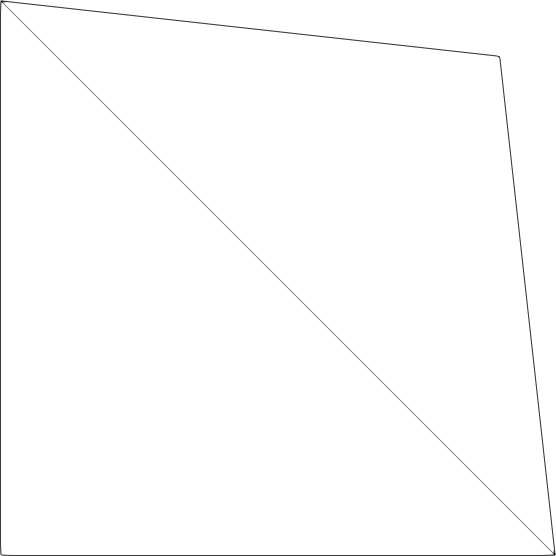
\includegraphics[height=3cm]{fig/1/1.png}
  \caption{Triangulation\_2}
  \label{fig:1-1}
\end{figure}
\begin{figure}[!htbp]
  \centering
  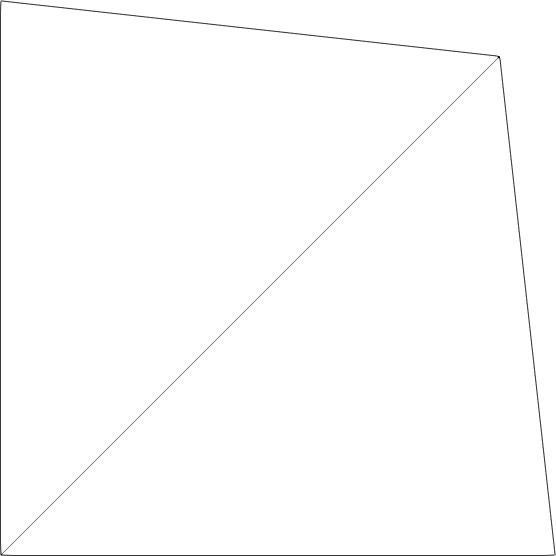
\includegraphics[height=3cm]{fig/1/2.png}
  \caption{Delaunay\_triangulation\_2}
  \label{fig:1-2}
\end{figure}
\begin{figure}[!htbp]
  \centering
  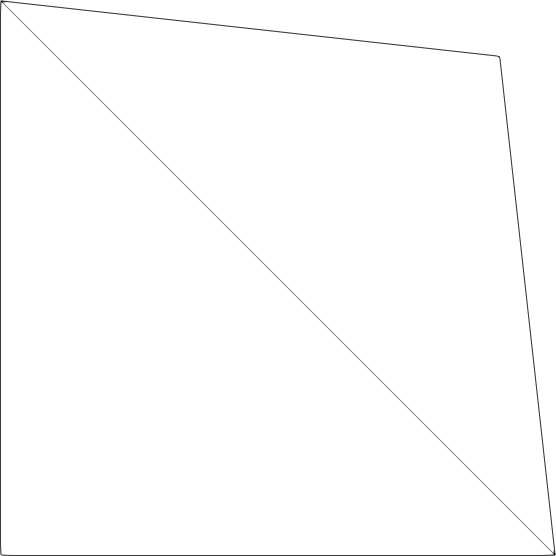
\includegraphics[height=3cm]{fig/1/3.png}
  \caption{Constrained\_Delaunay\_triangulation\_2}
  \label{fig:1-3}
\end{figure}
\begin{figure}[!htbp]
  \centering
  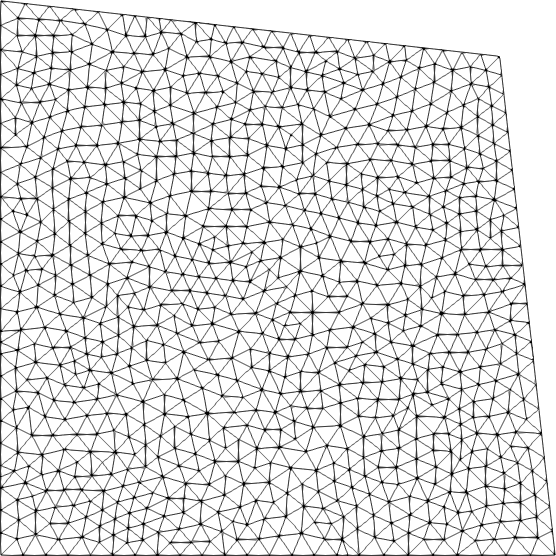
\includegraphics[height=3cm]{fig/1/4.png}
  \caption{Delaunay\_mesher\_2}
  \label{fig:1-4}
\end{figure}

当插入一个新点时,图\ref{fig:1-5}是Triangulation\_3,因此没有发生翻转。图\ref{fig:1-6}是Delaunay\_triangulation\_3,发生了翻转。图\ref{fig:1-7}采用OFF文件定义了多面体,多面体的面只能为三角形,进行了网格剖分。
\begin{figure}[!htbp]
  \centering
  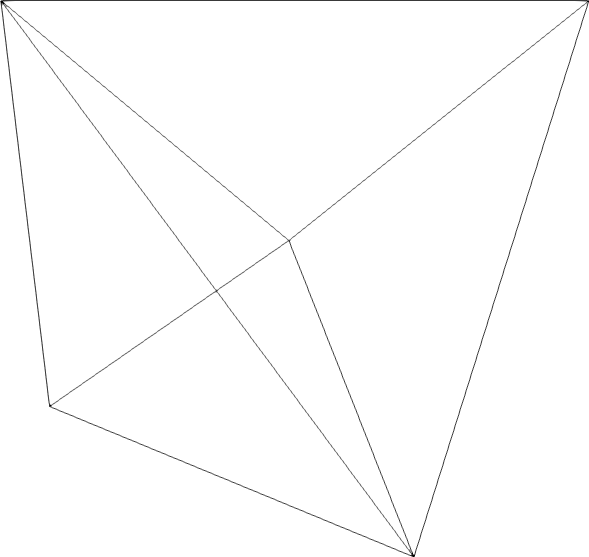
\includegraphics[height=3cm]{fig/1/5.png}
  \caption{Triangulation\_3}
  \label{fig:1-5}
\end{figure}
\begin{figure}[!htbp]
  \centering
  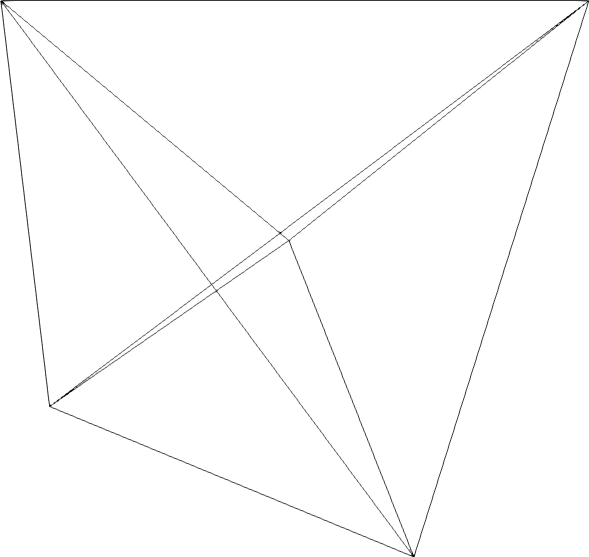
\includegraphics[height=3cm]{fig/1/6.png}
  \caption{Delaunay\_triangulation\_3}
  \label{fig:1-6}
\end{figure}
\begin{figure}[!htbp]
  \centering
  
\includegraphics[height=3cm]{fig/1/7.png}
  \caption{make\_mesh\_3}
  \label{fig:1-7}
\end{figure}


\subsection{Triangle}

Triangle是一个二维Delauany网格剖分的软件,是Jonathan Richard Shewchuk开发的。软件包括四个文件,triangle.h和triangle.c,可视化用的showme.c,以及一个c语言接口例子tricall.c。其中triangle.c中有main函数定义,可以直接从triangle.c编译成可执行程序,但是需要注释掉TRILIBRARY的定义,也可以将triangle.c编译成链接库,然后tricall.c调用链接库,将tricall.c编译成可执行程序。Triangle中给了一个例子,读取A.poly文件中数据进行网格剖分,结果会生成A.1.*的文件,然后用showme打开。在CMakeLists里将var设置成ON,是将triangle.c编译成可执行程序,设置成OFF,是将tricall.c编译成可执行程序。运行install.sh文件,编译安装后在bin文件夹中可以运行triangle$\_$run -p A进行测试,用showme A.poly打开查看。


\subsubsection{数据结构和算法}

\subsubsection{算例}

\subsection{Netgen}

\subsubsection{数据结构和算法}

\subsubsection{算例}

\subsection{Tetgen}

\subsubsection{数据结构和算法}

\subsubsection{算例}

\subsection{Gmsh}

\subsubsection{数据结构和算法}

\subsubsection{算例}

\subsection{OpenCASCADE}

\subsubsection{数据结构和算法}

\subsection{Slice2Mesh}

\subsubsection{数据结构和算法}

\subsubsection{算例}

\section{结构性网格}

\subsection{协调性网格}

\subsubsection{Clipper}

\subsubsection{RnD}

\subsubsection{数据结构和算法}

\subsubsection{算例}

\subsection{非协调性网格}

\subsubsection{数据结构和算法}

\subsubsection{算例}

\chapter{网格自适应性}

\chapter{网格并行}

\section{Metis}

\chapter{残余应力和变形}

\section{热弹塑性}

\section{小尺度热循环生死单元法}

\section{构件尺度固有应变法}
